\documentclass{article}
\usepackage[top=2cm, bottom=2cm, left = 2cm, right = 2cm]{geometry}
\usepackage{graphicx} % Required for inserting images
\usepackage{multirow}

\title{Algorytmy metaheurystyczne Lista 2}
\author{Bartłomiej Puchała}
\date{December 2023}

\begin{document}

\maketitle

\section{Simulated Annealing}
\subsection{Wybór parametrów}
\subsubsection{Wpływ zmiany temperatury początkowej na średnią długośc cyklu rozwiązania}
    \begin{figure}[h!]
        \centering
        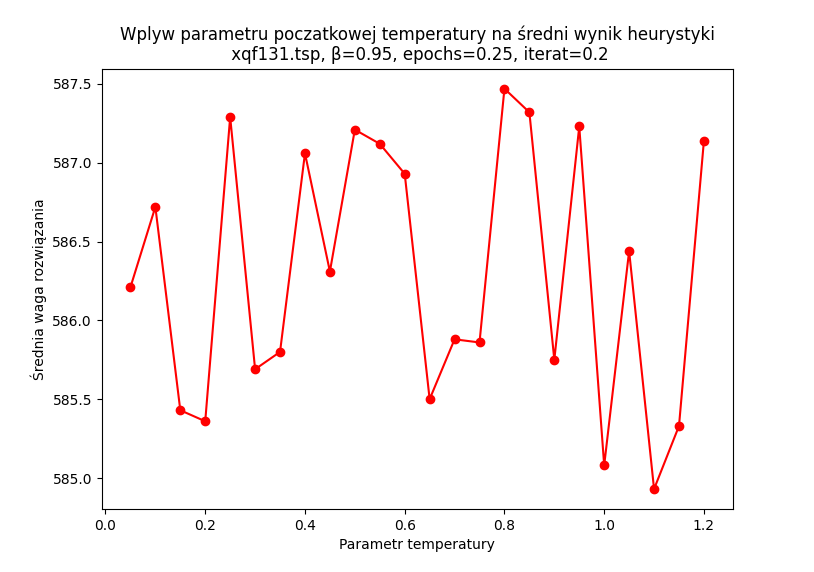
\includegraphics[height=9.5cm]{simulated_an_1.png}
    \end{figure}

    \begin{figure}[h!]
        \centering
        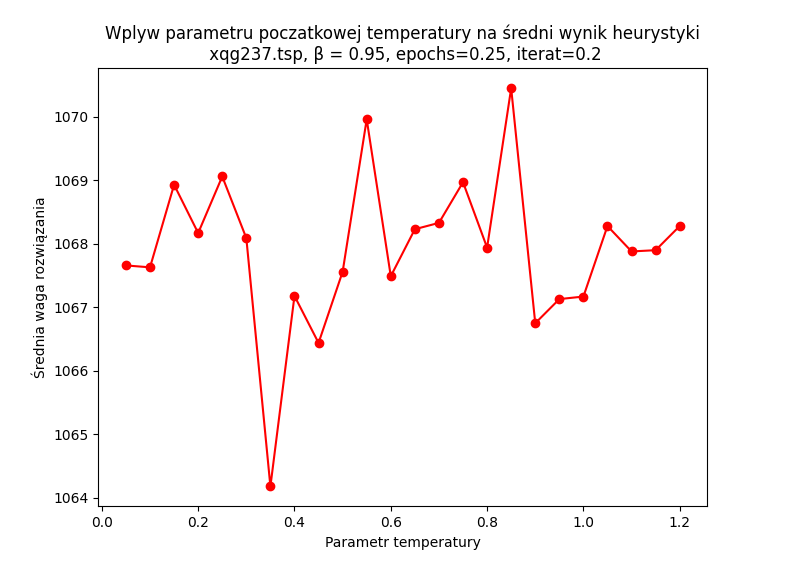
\includegraphics[height=9.5cm]{simulated_an_2.png}
    \end{figure}

\newpage

\subsubsection{Wpływ zmiany parametru obniżania temperatury na średnią długość cyklu rozwiązania}
    \begin{figure}[h!]
        \centering
        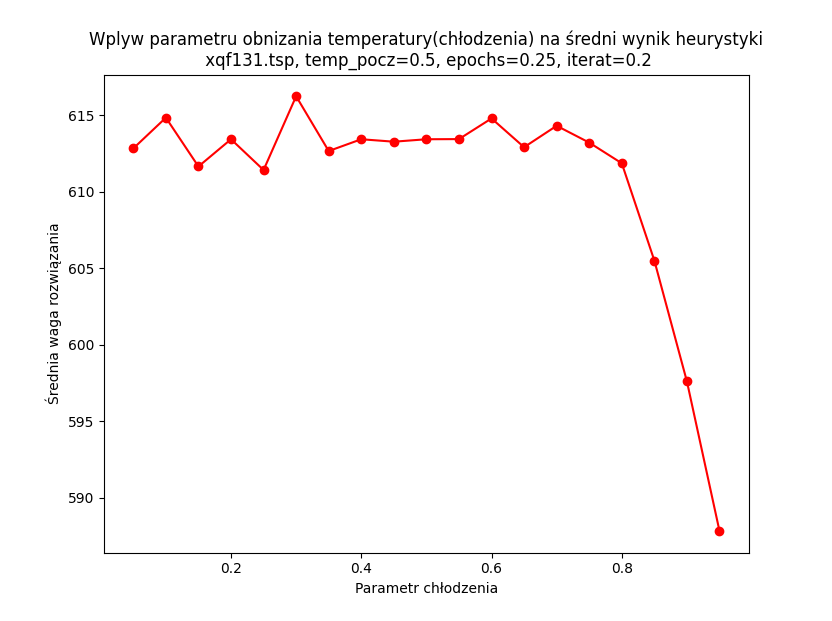
\includegraphics[height=9.5cm]{simulated_an_3.png}
    \end{figure}
        \begin{figure}[h!]
        \centering
        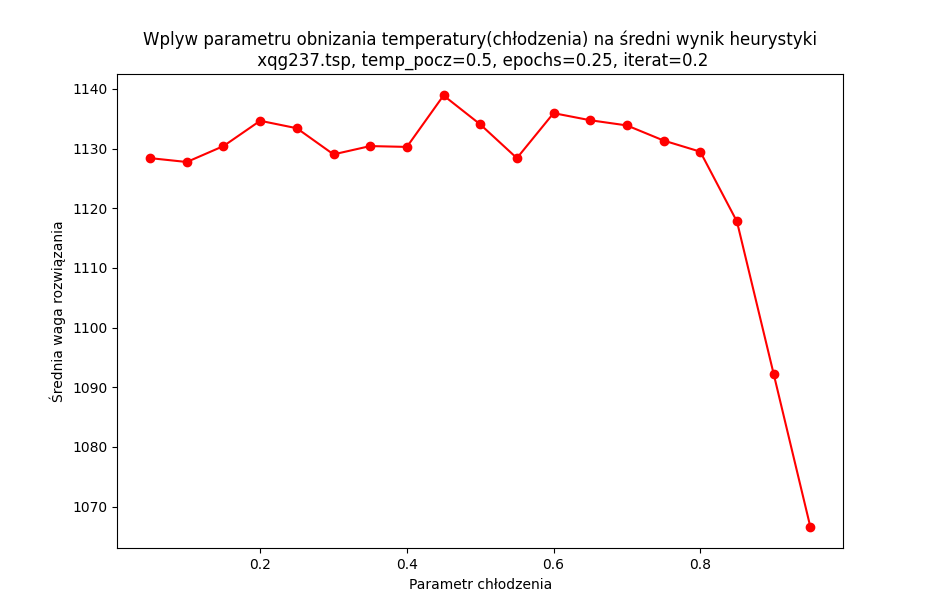
\includegraphics[height=9.5cm]{simulated_an_4.png}
    \end{figure}

\newpage

\subsubsection{Wpływ liczby prób przeprowadzanych w ramach jednej epoki na średnią długość cyklu rozwiązania}
    \begin{figure}[h!]
        \centering
        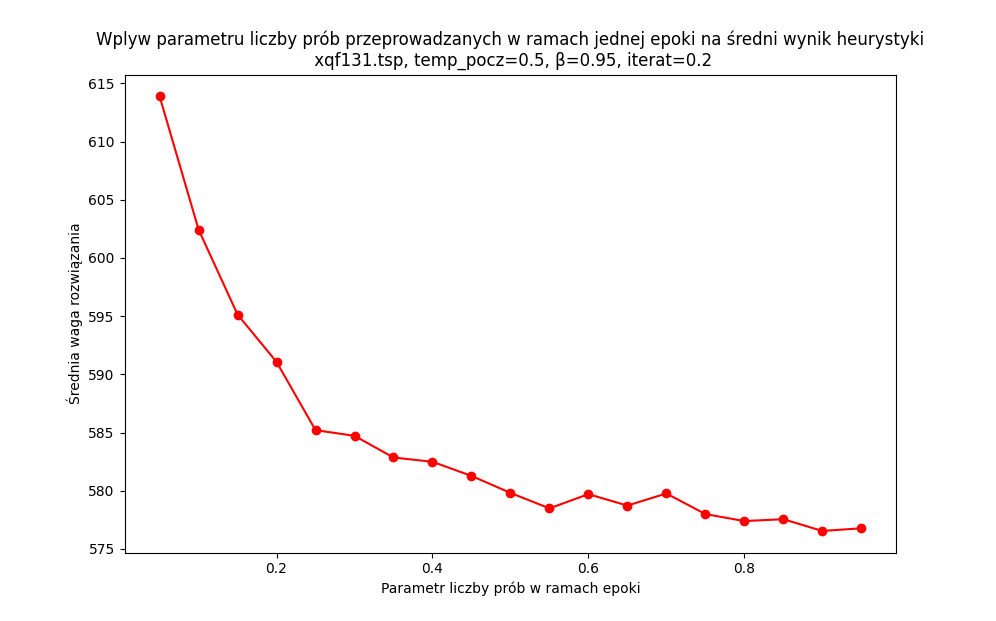
\includegraphics[height=9.5cm]{simulated_an_5.png}
    \end{figure}
        \begin{figure}[h!]
        \centering
        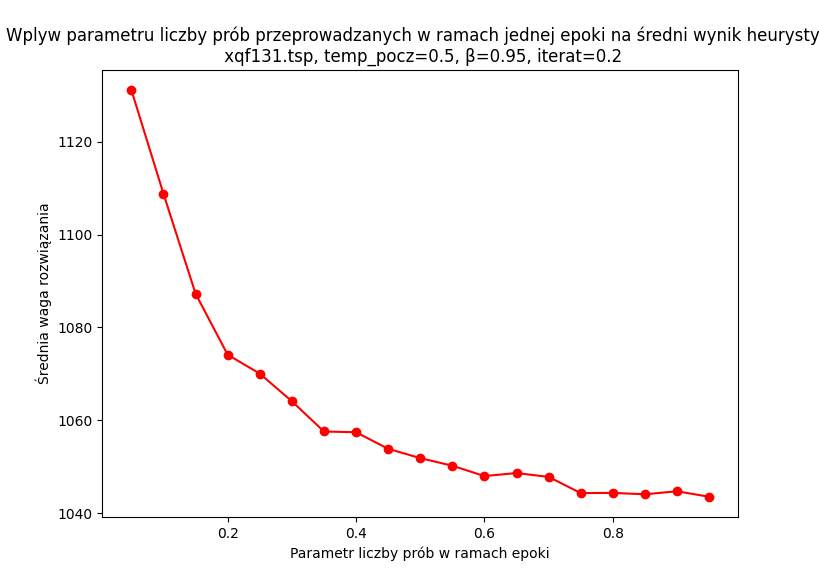
\includegraphics[height=9.5cm]{simulated_an_6.png}
    \end{figure}
    
\newpage

\subsubsection{Wpływ liczby prób przeprowadzanych w ramach jednej epoki na czas działania heurystyki}
    \begin{figure}[h!]
        \centering
        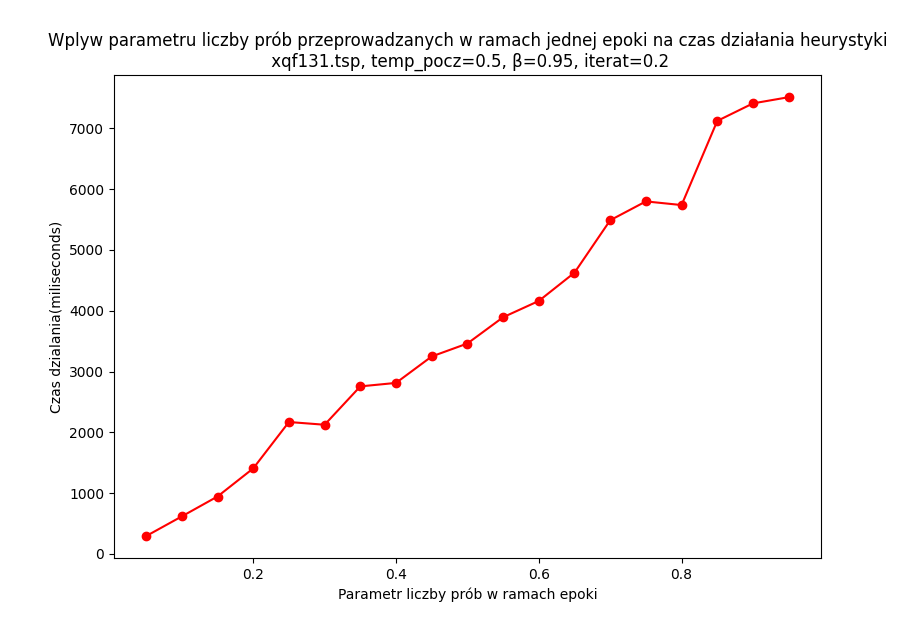
\includegraphics[height=9.5cm]{simulated_an_7.png}
    \end{figure}

\subsection{Ostateczne parametry}
\begin{itemize}
    \item Rozwiązanie początkowe: losowe
    \item Temperatura początkowa: $\alpha = 0.5$
    \item Chłodzenie: $\beta = 0.9$
    \item Długość epoki: $\gamma = 0.25$
    \item Liczba iteracji bez poprawy: $\delta = 0.15$
    \item Typ otoczenia: \texttt{INVERT}
\end{itemize}

\section{Tabu Search}
\subsection{Wybór parametrów}

\subsubsection{Wpływ długości listy tabu na średni wynik heurystyki}
    \begin{figure}[h!]
        \centering
        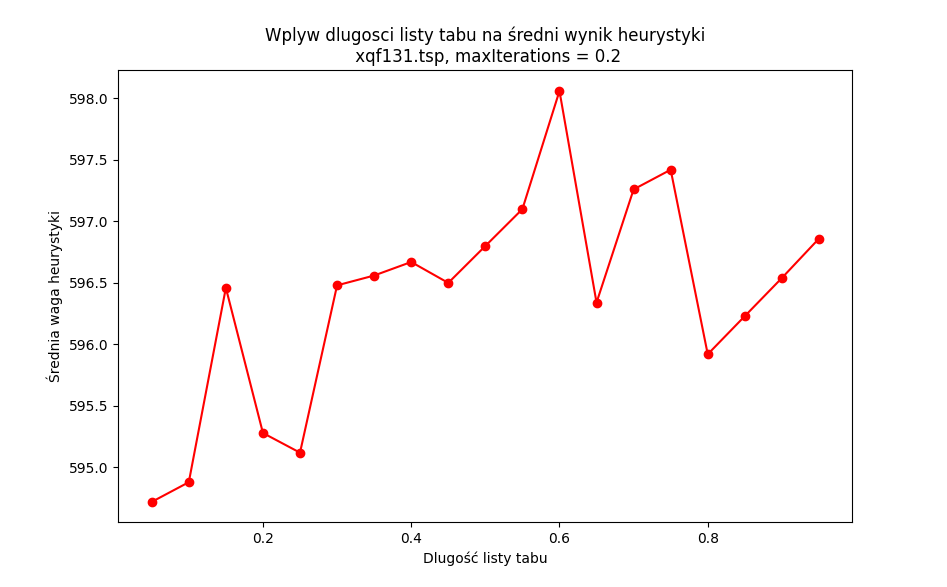
\includegraphics[height=9.5cm]{tabu_1.png}
    \end{figure}

\subsubsection{Ostateczne parametry}
\begin{itemize}
    \item Długość listy tabu: $\alpha = 0.12$
    \item Liczba iteracji bez poprawy: $\beta = 0.2$
    \item Typ otoczenia: \texttt{INVERT}
    \item Wybór otoczenia: pełne lub losowe
    \item Rozwiązanie początkowe: oparte o MST
\end{itemize}
    
\subsection{Analiza}

\newpage
\vspace{10pt}
\begin{center}
    \title{Wpływ wyboru rozwiazania poczatkowego oraz otoczenia na średnie wagi rozwiązań(100 powtórzeń)}
\end{center}

\begin{center}
    \begin{table}[h!]
        \centering
        \begin{tabular}{|c|c|c|c|c|}
            \hline 
            \multirow{2}{*}{Data} & \multicolumn{2}{|c|}{Random solution} & \multicolumn{2}{|c|}{MST solution} \\
            \cline{2-5} & Otoczenie pełne & Otoczenie losowe & Otoczenie pełne & Otoczenie losowe \\
            \hline
            xqf131 & 611.56 & 640.62 & 594.91 & 616.45 \\
            \hline
            xqg237 & 1096.2 & 1170.59 & 1061.2 & 1132 \\
            \hline
            pka379 & 1448 & 1492.79 & 1395.17 & 1449.65 \\
            \hline
            bcl380 & 1825.4 & 1888.33 & 1716.4 & 1794.12 \\
            \hline
        \end{tabular}
    \end{table}
\end{center}
\vspace{10pt}

\begin{center}
    \title{Wpływ wyboru rozwiazania poczatkowego oraz otoczenia na czas działania algorytmu}
\end{center}


\begin{center}
    \begin{table}[h!]
        \centering
        \begin{tabular}{|c|c|c|c|c|}
            \hline 
            \multirow{2}{*}{Data} & \multicolumn{2}{|c|}{Random solution} & \multicolumn{2}{|c|}{MST solution} \\
            \cline{2-5}
            \cline{2-5} & Otoczenie pełne & Otoczenie losowe & Otoczenie pełne & Otoczenie losowe \\
            \hline
            xqf131 & 0.912 & 0.063 & 0.208 & 0.027 \\
            \hline
            xqg237 & 8.723 & 0.21 & 2.494 & 0.174 \\
            \hline
            pka379 & 57.21 & 0.875 & 13.807 & 0.413 \\
            \hline
            bcl380 & 64.21 & 1.11 & 14.597 & 0.577 \\
            \hline
        \end{tabular}
    \end{table}
\end{center}


\section{Wyniki}
\begin{table}[h!]
    \centering
    \begin{tabular}{|c|c|c|c|c|c|c|c|}
        \hline
        \multirow{2}{*}{Data} & \multirow{2}{*}{Optimum} & \multicolumn{2}{|c|}{Local Search} & \multicolumn{2}{|c|}{Simulated Annealing}  & \multicolumn{2}{|c|}{Tabu Search}  \\
        \cline{3-8}
        & & śr. waga & min. waga & śr. waga & min. waga & śr. waga & min. waga \\
        \hline
        xqf131 & 564 & 612 & 583 & 589.44 & 569 & 611.52 & 588 \\
        \hline
        xqg237 & 1019 & 1118 & 1063 & 1073.08 & 1045 & 1103.33 & 1064 \\
        \hline
        pma343 & 1368 & 1483 & 1423 & 1413.76 & 1388 & 1440.32 & 1410 \\
        \hline
        pka379 & 1332 & 1446 & 1396 & 1377.07 & 1347 & 1399.26 & 1383 \\
        \hline
        bcl380 & 1621 & 1818 & 1740 & 1719.28 & 1674 & 1739.28 & 1709 \\
        \hline
        pbl395 & 1281 & 1427 & 1365 & 1362.54 & 1323 & 1377.8 & 1352 \\
        \hline
        pbk411 & 1343 & 1489 & 1421 & 1425.52 & 1387 & 1433.3 & 1405 \\
        \hline
        pbn423 & 1365 & 1522 & 1456 & 1449.55 & 1407 & 1468.4 & 1440 \\
        \hline
        pbm436 & 1443 & 1611 & 1536 & 1528.38 & 1472 & 1563.5 & 1535 \\
        \hline
        xql662 & 2513 & 2827 & 2727 & 2673.51 & 2606 & 2699.4 & 2673 \\
        \hline
        xit1083 & 3558 & 4012 & 3908 & 3825.5 & 3746 & 3909.11 & 3768 \\
        \hline
        icw1483 & 4416 & 5121 & 4942 & 4749.04 & 4680 & 4739.7 & 4733 \\
        \hline
        djc1785 & 6115 & 6857 & 6742 & 6545.1 & 6460 & 6470.7 & 6450 \\
        \hline
        dcb2086 & 6600 & 7499 & 7400 & 7129.6 & 7074 & 7171.7 & 7153 \\
        \hline
        pds2566 & 7643 & 8705 & 8562 & 8225 & 8151 & 8377 & 8255 \\
        \hline
    \end{tabular}
    \caption{Porównanie wyników metaheurystyk: Local Search, Simulated Annealing i Tabu Search.}
\end{table}

\end{document}
